We will our connectivity dataset and crawl across it to find a particularly great subgraph.  If time allows, we will attempt to restore and expand the incomplete information within this subgraph.  We will then create overlays of this subgraph using different user attributes.  We will analyze the directional nature of these subgraph overlays.

\begin{figure}
 \centering
 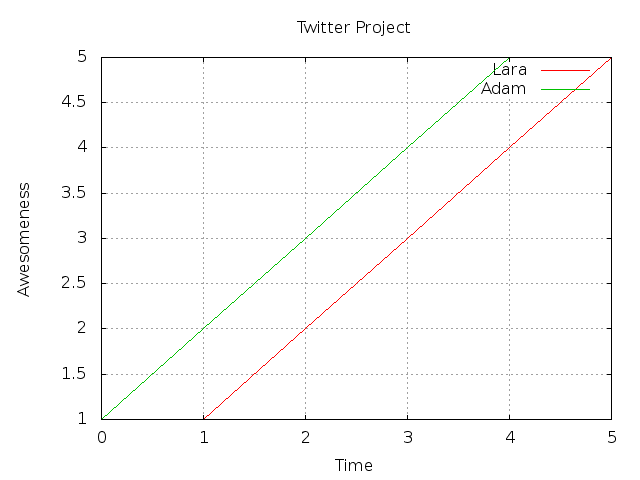
\includegraphics[bb=0 0 640 480,scale=.25]{./images/evidence.png}
 % evidence.png: 640x480 pixel, 72dpi, 22.58x16.93 cm, bb=0 0 640 480
 \caption{This is what a graph looks like.}
 \label{Figure 1:}
\end{figure}

\subsection{Assessing the validity of our subgraph}